\documentclass[man]{apa7}
\usepackage[T1]{fontenc}
\usepackage[american]{babel}
\usepackage[style=apa,backend=biber]{biblatex}
\usepackage{csquotes}
\addbibresource{CountDominance.bib}

\title{Relative importance analysis for count regression models}
\author{Joseph N. Luchman}
\affiliation{Fors Marsh}
\leftheader{Luchman}
\shorttitle{Count Model Dominance}
\authornote{\addORCIDlink{Joseph N. Luchman}{0000-0002-8886-9717}. The author has read and approved the final version of the manuscript, has no conflicts of interest with respect to his authorship or the publication of this article, and did not receive or benefit from fundings of this article.}

\abstract{
	Count variables are common in behavioral science as an outcome. 
	Count regression models (CRMs), such as Poisson regression, are recommended when analyzing count variables but can be challenging to interpret given their non-linear functional form. 
	I recommend relative importance analysis as a method to use in interpreting CRM results. 
	This work extends on past research by describing an approach to determining the importance of independent variables in CRMs using dominance analysis (DA). 
	In this manuscript, I review DA as a relative importance method, recommend a pseudo-$R^2$ to use with CRM-based DA, and outline the results of an analysis with simulated data that uses the recommended methodology. 
	This work contributes to the literature by extending DA to CRMs and provides a thoroughly documented example analysis that researchers can use to implement the methodology in their research.
}

\keywords{Dominance Analysis, Relative Importance, Poisson Regression, R-square, Negative Binomial Regression, Count Data}
	
\begin{document}

\maketitle

	Behavioral scientists often use how many times a behavior is observed as an outcome to answer research questions. 
	Such behavior counts arise from many different sources among aggreates or collectives of people and individuals over time.
	Aggregate behavior counts used in the literature include the number of organizations adopting a specific practice in a week \parencite{naumovska2021strength} and number of divestitures organizations make in a year \parencite{bettinazzi2021stakeholder}. 
	Individual-level behavior counts used in the literature include the number of scientific articles published in a year among scholars \parencite{rotolo2013does} or number of errors that resulted in an accident in the last three months among medical doctors \parencite{naveh2015active}.
	Behavior counts such as the above examples are valuable outcomes given that behavioral science concepts are often defined terms of behavior \parencite[e.g., job performance;][]{motowidlo2003job} and strategies to validate outcomes often use observable behavior as an outcome \parencite[e.g., criterion-oriented validity;][]{cronbach1955construct}.
	
	However valuable as outcomes, behavior counts as a dependent variable/DV in data analysis require the use of specialized tools.
	The recommended data analysis strategy with behavior counts uses regression models designed for non-negative integer or count distributions \parencite[e.g.,][]{blevins2015count}.
	These count regression models/CRMs include the Poisson regression/PR and negative Binomial regression/NBR models.
	Both PR and NBR are commonly used in the behavioral science literature and implemented in many data analytic software environments.
	
	CRMs are generalized linear models that transform the predictive equation to ensure that predicted values stay in the range of the DV.
	CRMs use an exponential or log-linear transformation that has the form $y = e^{\beta}$. 
	Thus, the predictive equation represented by $\beta$ requires back-transformation using a natural logarithm in order to obtain a predicted count value.
	This log-linear transformation ensures that the linear predictrd values can take on any real number yet, when back-transformed into predicted counts, will have a lower bound of 0.
	
	CRM results are challenging to interpret directly.
	This is because CRM coefficients describe how the natural logarithm of the DV changes given a 1 unit change to an independent variable/IV. 
	When back-translated through an exponential function, CRM coefficients are known as incidence rate ratios and describe the percentage change in the DV per unit change to the IV.
	Because IRRs describe percentage change, CRM coefficients produce predicted values that are relative or change in their magnitude over the continuum of the DV.
	For example, a CRM coefficient does not differentiate between a change from 1 predicted behavior to 2 and 5 predicted behaviors to 10. 
	Despite the noteworthy difference in the absolute number of behaviors in both examples, each describe a 100\% increase.
		
	Model post-estimation methods such as graphing estimated marginal means are useful interpretive tools for log-linear CRMs as they help to contextualize the CRMs' predicted values.
	Another increasingly common model post-estimation tool used to contextualize model predictions is relative importance analysis \parencite{tonidandel2011relative}. 
	Relative importance analysis is used to compare how each IV in the model contributes to a model fit metric such as the $R^2$ and is commonly implemented using dominance analysis/DA \parencite{azen2003dominance}.
	
	Published methodological work has extended DA from the linear regression model/LRM on which it was originally developed, to other linear models including binary \parencite{azen2009using}, ordered, and multinomial logit models \parencite{luchman2014relative}.	
	This work extends DA to CRMs and, in so doing, makes two contributions to the literature.
	This work first reviews DA as a relative importance methodology, recommends using a specific pseudo-$R^2$ statistic for CRM-based DA, and implements a data analytic example of DA.

	Second, this paper extends on the work of Blevins, Tsang, and Spain \parencite*{blevins2015count} who review and offer multiple recommendations for the application of CRMs to research questions in behavioral science. 
	Blevins et al. describe model and analytic details about the PR and NBR models and provide a flowchart that researchers can use to identify which CRM might be best to choose for their data analysis.
	In this work, I extend on their review to add an in-depth discussion of DA and its role as a post-estimation methodology.
	DA extends on the interpretation of coefficients to describe how the coefficients, when applied to the observed data, improve model-to-data fit in predicting the count DV.

	I begin the manuscript with a discussion of the conceptual background of DA.
	The conceptual discussion of DA focuses on outlining three different levels of dominance between IVs, how these levels of dominance are determined in the data, and what each level of dominance means in terms of IV importance.
	The next section recommends a fit metric to apply to CRMs for the purpose of determinining importance using DA.
	In this CRM focused section, I draw parallels between the explained variance $R^2$ used by the LRM as a fit metric and an analogous fit metric for CRMs that is particularly useful for DA.
	Finally, I describe an extensive data analytic example.
	This final section uses simulated data to estimate a PR model and a PR model-based DA where the methods described in the previous two sections are applied.
		
\section{Dominance Analysis}

	Behavioral scientists have used many methods over the years to determine how important an IV is in a LRM \parencite[see reviews in][]{gromping2007estimators, johnson2004history}.
	Methods for determining the importance of an IV have ranged from the use of a correlation coefficient between the IV and DV, to the IV's standardized regression coefficient, to the increment the IV makes to the $R^2$ over and above other IVs.
	These methods, however informative in specific circumstances, make assumptions about an IV's contribution to prediction.
	These methods assume in some cases that an IV's contribution should not be adjusted for other IVs (i.e., the correlation coefficient) and in other cases that the adjustment should occur only after all other IVs are included (i.e., incremental $R^2$, standardized coefficient).
	In most situations, IV inclusion ordering is arbitrary and as opposed to choosing one approach or the other, recommended importance methods should account for different bi- and multivariate relationships with the DV \parencite{johnson2004history}.
	The most conceptually useful importance methods then produce determinations that are independent of IV inclusion order.
	
	DA is a method for determining IV importance independent of inclusion order that was originally developed for the LRM by Budescu \parencite*{budescu1993dominance}.
	DA extended on previously proposed methods by defining importance in terms of pairwise IV comparisons across $R^2$ values associated with multiple sub-models.
	An LRM with $p$ IVs produces total of $2^p$ sub-models corresponding to all possible combinations of IVs included or excluded from estimation.
	DA achieves order independence in the importance determiniations it makes by comparing the $R^2$ values associated with the two focal, comparison IVs' across all sub-models that include combinations of non-focal, other IVs. 
	A non-focal IV sub-model is one that contains a distinct subset of the $p - 2$ IVs that are not the focus of the comparison.
	The $\emptyset$ or a sub-model that includes no non-focal IVs, is also a possible sub-model used in these comparisons.	
	In this way, the dominance comparisons do not depend on the order of IV inclusion and require that one of the focal, comparison IVs obtain a higher $R^2$ value than the other focal IV across all sub-models---that is, irrespective of the order in which the IV is included in the model.
	
	As an example of how the dominance comparison is implemented, consider a model with 4 IVs: $IV_x$, $IV_z$, $IV_w$ and $IV_v$ predicting $Y$.
	If I am comparing $IV_x$ and $IV_z$, there would be a total of four possible $R^2$ comparisons, each of which is reported below in Table \ref{tab:exdom}.
	In each comparison, the subscripted model indicates the LRM prediction equation in symbolic form.
	The terms in braces include the other, non-focal IV subset across which both of the focal, comparison IVs are being evaluated.
	$IV_x$ dominates $IV_z$ only when all the $R^2$ values for sub-models that include $IV_x$ are greater than the $R^2$ values for sub-models that include $IV_z$.
	The dominance comparisons described in this section are known as complete dominance and are recognized as the most stringent, or hardest to achieve, dominance designation that an IV can have over another IV \parencite{azen2003dominance}.	

		\begin{table}[h!]
			\centering
			\caption{\centering Example Dominance Comparisons}
			\begin{tabular}{ l | l l }
				
				& Sub-model with $IV_x$ & Sub-model with $IV_z$ \\
				\hline
				Across null set/no other IVs & $R^2_{Y \sim IV_x + \{\emptyset\}}$ & $R^2_{Y \sim IV_z+ \{\emptyset\} }$ \\
				Comparing across $IV_w$ & $R^2_{Y \sim IV_x + \{IV_w\}}$ & $R^2_{Y \sim IV_z + \{IV_w\}}$ \\
				Comparing across $IV_v$ & $R^2_{Y \sim IV_x + \{IV_v\}}$ & $R^2_{Y \sim IV_z + \{IV_w\}}$ \\
				Comparing across both $IV_w$ and $IV_v$ & $R^2_{Y \sim IV_x + \{IV_w + IV_v\}}$ & $R^2_{Y \sim IV_z + \{IV_w + IV_v\}}$ \\
				\hline
		\end{tabular}
		\label{tab:exdom}
	\end{table}
	
	\subsection{Complete Dominance}
	
	Complete dominance is the most stringent of the dominance designations as it is a difficult designation for an IV to achieve over another.
	Complete dominance is difficult to achieve as it involves direct comparisons between IV pairs across multiple sub-model $R^2$ values and is non-compensatory; all sub-model $R^2$ value comparisons must show that one IV has a larger value than the other IV or the designation will fail to be achieved.
	
	The process for determining complete dominance between a pair of IVs, for example $IV_x$ and $IV_z$, with an arbitrary number of non-focal IVs in the model ($p - 2$) proceeds as:
	\begin{equation}
		IV_x \, D \, IV_z \quad if \quad 2^{p-2} = \sum^{2^{p-2}}_{j=1} \Biggr\{ 
		\begin{array}{l}
			if \ R^2_{Y \sim IV_x + \{u_j\}} > R^2_{Y \sim IV_z + \{u_j\}} \ then \ 1 \\
			else \ 0 
		\end{array}
		\label{eq:cptdom}
	\end{equation}
	Where $u_j$ is a distinct subset of the other $p - 2$ IVs.
	As in Table \ref{tab:exdom}, the braces surrounding $u_j$ indicate that it is a subset of non-focal IVs.
	The $D$ in this case is a designation indicating complete dominance of $IV_x$ over $IV_z$.
	Ultimately, if $IV_x$ completely dominates $IV_z$ as is outlined in Equation \ref{eq:cptdom}, $IV_x$ is clearly and unconditionally better than $IV_z$ in terms of explaining variance in $Y$ given the LRM from which all sub-models were derived.	
	
	Because complete dominance is a difficult criterion to achieve in comparing IV pairs, alternative and more compensatory, dominance designations have been proposed to provide more ways to compare the predictive usefulness of IVs against one another.
	As I will discuss, the alternative dominance designations involve averaging the $R^2$ increment values associated with each IV and determining importance by comparing those average values.
	
	\subsection{Conditional Dominance}
	
	A less stringent dominance designation between IV pairs than complete dominance is called conditional dominance.
	Conditional dominance relaxes the stringency of the comparisons across pairs of IVs by evaluating how each IV contributes to the $R^2$, on average, when they are included in every relative position in the model.
	
	By comparing averages of $R^2$ increments by relative position, conditional dominance allows some sub-models with higher $R^2$ increment values at a specific inclusion order for $IV_x$ compared to $IV_z$ to compensate for sub-models with lower $R^2$ increment values for $IV_x$ compared to $IV_z$ at that same order.
	This compensatory property of the averages by inclusion order makes conditional dominance a less stringent criterion and makes it more likely to obtain a dominance designation.
	
	The average increments to the $R^2$ used to determine conditional dominance are known as conditional dominance statistics.
	Because each IV can be included at any relative position in the model, in a model with $p$ IVs, each IV will have $p$ conditional dominance statistics to compare to another IV.
	Extending on Table \ref{tab:exdom}, determining conditional dominance between $IV_x$ and $IV_z$ would involve all four different conditional dominance statistics, the computation of which are outlined below in Table \ref{tab:excdl}.
	
	\begin{table}[h!]
		\centering
		\caption{\centering Example Conditional Dominance}
		\begin{tabular}{ l | l l }
			Comparing at & Average with $IV_x$ & Average with $IV_z$ \\
			\hline
			One IV & $\Delta R^2_{Y \sim IV_x + \{\emptyset\}}$ & $\Delta R^2_{Y \sim IV_z + \{\emptyset\}}$ \\
			\hline
			& $(\Delta R^2_{Y \sim IV_x + \{IV_w\}} + $ & $(\Delta R^2_{Y \sim IV_z + \{IV_w\}} + $ \\
			Two IVs & $\Delta R^2_{Y \sim IV_x + \{IV_v\}} + $ & $\Delta R^2_{Y \sim IV_z + \{IV_v\}} + $ \\
			& $\Delta R^2_{Y \sim IV_x + \{IV_z\}})\frac{1}{3}$ & $\Delta R^2_{Y \sim IV_z + \{IV_x\}})\frac{1}{3} $ \\
			\hline
			& $(\Delta R^2_{Y \sim IV_x + \{IV_w + IV_v\}} + $ & $(\Delta R^2_{Y \sim IV_z + \{IV_w + IV_v\}} + $ \\
			Three IVs & $\Delta R^2_{Y \sim IV_x + \{IV_w + IV_z\}} + $ & $\Delta R^2_{Y \sim IV_z + \{IV_w + IV_x\}} + $ \\
			& $\Delta R^2_{Y \sim IV_x - \{IV_v + IV_z\}})\frac{1}{3}$ & $\Delta R^2_{Y \sim IV_z + \{IV_v + IV_x\}})\frac{1}{3}$ \\
			\hline
			Four IVs & $\Delta R^2_{Y \sim IV_x + \{IV_w + IV_v + IV_z\}}$ & $\Delta R^2_{Y \sim IV_z + \{IV_w + IV_v + IV_x\}}$ \\
			\hline
		\end{tabular}
		\label{tab:excdl}
	\end{table}
	
	The $\Delta$ used in Table \ref{tab:excdl} indicates that the $R^2$ value is an increment made by the focal IV beyond the subset of non-focal IVs in braces.
	Note that the conditional dominance statistics use $R^2$ increments from subsets that include all other non-focal IVs.
	Hence, conditional dominance comparisons between two IVs will include increments from the IV against which they are being compared in their average value.
	This is a noteworthy difference from complete dominance designations that do not use sub-model $R^2$ values that include the IV against which the focal IV is being compared.
	
	The process of computing conditional dominance statistics for $IV_x$ with $i$ IVs in the sub-model is defined as in Equation \ref{eq:cdlst} below.
	\begin{equation}
		C^{i}_{IV_x} = \frac{\sum^{k_i}_{g=1} \Delta R^2_{IV_x + \{o_g\}}}{k_g}
		\label{eq:cdlst}
	\end{equation}
	Where $k_i$ is the number of combinations of size $i$ given $p$ IVs and $o_g$ is a distinct subset of the $p - 1$ IVs of size $i - 1$ that are included in the sub-model.	
	Determining conditional dominance between $IV_x$ and $IV_z$ proceeds as in Equation \ref{eq:cdldom}.
	\begin{equation}
		IV_x \ D_c \ IV_z \quad if \quad p = \sum^p_{i=1} \Biggl\{ 
		\begin{array}{l}
			if \ C^{i}_{IV_x} > C^{i}_{IV_z} \ then \ 1 \\ 
			else \ 0 
		\end{array}
		\label{eq:cdldom}
	\end{equation}
	Where $D_c$ is a designation indicating conditional dominance of $IV_x$ over $IV_z$.	
	When $IV_x$ does not completely but does conditionally dominate $IV_z$, $IV_x$ is generally better than $IV_z$ for explaining variance in $Y$ given the underlying LRM irrespective of inclusion order in the model.
	Conditional dominance thus suggests that $IV_x$'s explanatory value is generally higher than $IV_z$ when considering their values at the same inclusion orders.
	
	Conditional dominance between an IV pair is less stringent than complete dominance but can still be a difficult designation to meet in models with a great deal of between-IV overlap.
	As a result, a third dominance designation was developed that involves yet another averaging step as is described in the next section.
	
	\subsection{General Dominance}
	
	The least stringent dominance designation between IV pairs is called general dominance.
	General dominance further relaxes the stringency of the comparisons between IV pairs by changing the focus from comparing average increments grouped by the number of IVs in a sub-model to the arithmetic average of these averages.
	General dominance is then the average of the conditional dominance statistics for each IV.
	By averaging over conditional dominance statistics, general dominance allows higher contributions at specific numbers of IVs in the sub-model to compensate for lower contributions at other numbers of IVs in the sub-model. 
	The values generated by general dominance will, in almost all cases, produce a dominance designation between the pair of IVs.
	
	The averaged conditional dominance statistics computed for determining general dominance are known as general dominance statistics. 
	Table \ref{tab:exgen} shows the general dominance statistic computation for $IV_x$ and $IV_z$.
	This computation incorporates all the values in Table \ref{tab:excdl} but summed into a single statistic.
	
		\begin{table}[h!]
		\centering
		\caption{\centering Example General Dominance}
		\begin{tabular}{ l l }
			Average with $IV_x$ & Average with $IV_z$ \\
			\hline
			$\Delta R^2_{Y \sim IV_x + \{\emptyset\}}\frac{1}{4} + $ & $\Delta R^2_{Y \sim IV_z + \{\emptyset\}}\frac{1}{4} +$ \\
			$(\Delta R^2_{Y \sim IV_x + \{IV_w\}} + $ & $(\Delta R^2_{Y \sim IV_z + \{IV_w\}} + $ \\
			$\Delta R^2_{Y \sim IV_x + \{IV_v\}} + $ & $\Delta R^2_{Y \sim IV_z + \{IV_v\}} + $ \\
			$\Delta R^2_{Y \sim IV_x + \{IV_z\}})\frac{1}{12} + $ & $\Delta R^2_{Y \sim IV_z + \{IV_x\}})\frac{1}{12} + $ \\
			$(\Delta R^2_{Y \sim IV_x + \{IV_w + IV_v\}} + $ & $(\Delta R^2_{Y \sim IV_z + \{IV_w + IV_v\}} + $ \\
			$\Delta R^2_{Y \sim IV_x + \{IV_w + IV_z\}} + $ & $\Delta R^2_{Y \sim IV_z + \{IV_w + IV_x\}} + $ \\
			$\Delta R^2_{Y \sim IV_x - \{IV_v + IV_z\}})\frac{1}{12} + $ & $\Delta R^2_{Y \sim IV_z + \{IV_v + IV_x\}})\frac{1}{12} +$ \\
			$\Delta R^2_{Y \sim IV_x + \{IV_w + IV_v + IV_z\}}\frac{1}{4}$ & $\Delta R^2_{Y \sim IV_z + \{IV_w + IV_v + IV_x\}}\frac{1}{4}$ \\
			\hline
		\end{tabular}
		\label{tab:exgen}
	\end{table}

	As is implied by the computations in Table \ref{tab:exgen}, general dominance statistics are a weighted average of the individual increments to the $R^2$s and is defined for $IV_x$ in Equation \ref{eq:genst}.
	\begin{equation}
		C_{IV_x} = \frac{\sum^{p}_{i=1} C^i_{IV_x}}{p}
		\label{eq:genst}
	\end{equation}
	Using the general dominance statistics computed in Equation \ref{eq:genst}, determining whether $IV_x$ generally dominates $IV_z$ is proceeds as in Equation \ref{eq:gendom}.
	\begin{equation}
		IV_x \ D_g \ IV_z \quad if \quad C_{IV_x} > C_{IV_z}
		\label{eq:gendom}
	\end{equation}
	Where $D_g$ is a designation indicating general dominance of $IV_x$ over $IV_z$.	
	When $IV_x$ does not completely or conditionally but does generally dominate $IV_z$, $IV_x$ is generally better than $IV_z$ for explaining variance in $Y$ given the underlying LRM but is sensitive to inclusion order in the model.
	General dominance thus suggests that $IV_x$'s predictive usefulness is, on average, better than $IV_z$ and that it is more important when not directly considering the effects of IV inclusion order.
	
	Note that the general dominance statistic values, when summed across the $p$ IVs, equals the sub-model $R^2$ when all $p$ IVs are included.
	This is a useful feature of the general dominance statistics that, as has been discussed in other reviews \parencite{gromping2007estimators,johnson2004history}, ties this method to earlier work on IV importance which focused on the decomposition of the $R^2$ statistic.

	In the sections above, I have provided a brief discussion of the conceptual development of the DA method, reviewed how DA statistics are computed, and reviewed how importance for IVs is determined.
	In the section below, I transition from a broad outline of DA to a more targeted discussion on application of DA to CRMs.
	The focus of the next section is on a discussion of CRM-based DA with attention to considering which fit statistic should be used when applying DA to CRMs.
	
\section{Applying Dominance Analysis to Count Regression Models}

	A complication of applying DA to CRMs is that the literature on DA has generally focused on how to apply the method to the LRM with the variance explained $R^2$ as a fit statistic.
	Given the semi-continuous nature of count DVs and that the predicted values from CRMs are typically in the form of a non-negative rational number, it is possible to use the explained variance $R^2$ when determining importance with a CRM.
	
	Although the variance explained $R^2$ could be applied to CRMs, there are good conceptual reasons to choose another fit statistic. 
	In the section below, I provide a rationale for the choice of a different metric, the deviance $R^2$ or $R^2_{DEV}$, that better reflects the criteria underlying how CRMs fit to data. 
	
	\subsection{Count Regression Fit Statistic: Deviance $R^2$} 
	
	Statistical models are fit using information about the data as applied to a probability distribution to find their most likely parameter values.
	A fit statistic applied to evaluating the fit of a statistical model to data is also most useful when the computation of the statistic is conceptually aligned with the model that it is being used to evaluate.
	Thus, choosing a fit statistic that matches the underlying fitting criterion of statistical model's probability distribution will best reflect how the model fits to data.
	
	Consider that the explained variance $R^2$ is computed as $\frac{\sum (\bar{Y} - \hat{Y})^2}{\sum (Y - \bar{Y})^2} = \frac{SS_{model}}{SS_{total}}$ or the ratio of the variance of the predicted values (i.e., the model sums of squares; $SS_{model}$) over the variance of the predicted values (i.e., the total sums of squares; $SS_{total}$).
	The LRM is based on a Normal probability distribution and uses least-squares as its fitting criterion.
	Least squares seeks to minimize $SS_{residual} = \sum (Y - \hat{Y})^2$ or the residual sums of squares between the predicted values from the LRM and the observed DV. 
	The $SS_{residual} = SS_{total} - SS_{model}$ and thus the explaned variance $R^2$ can also be computed as $1 - \frac{SS_{residual}}{SS_{total}}$.
	The explained variance $R^2$ is then closely tied to the LRM and its fitting criterion.
	It is important to note that the computation used to obtain the $SS_{residual}$ is also known as the deviance ($DEV$) for the Normal distribution as it describes how the model's predictions deviate from observed values \parencite{mccullagh2019generalized}.
	The $SS_{residual}$ is thus a $DEV_{model}$ or a model deviance for the LRM.
	
	The PR follows the Poisson distribution and the NBR follows the negative Binomial distribution--both of which are probability distributions meant for discrete data like non-negative counts.
	For example, the deviance for PR and a special case of the NBR\footnote{
		This special case is the NBR estimated using a quasi-likelihood method. 
		Maximum likelihood methods require a more complex form given the estimation of the $\alpha$/$\delta$ parameter.} 
	is $\sum Y\ln \frac{Y}{\hat{Y}} - (Y - \hat{Y})$. 
	Note that this PR-focused deviance value differs from the Normal distribution deviance in that it tends to penalize underprediction more than overprediction.
	The extra penalties assigned to underprediction are consistent with the truncated, semi-continuous nature of count DVs in that they cannot go below 0 and, thus, tend to be penalized more heavily toward the conceptual lower bound of the distribution.
	By contrast, Normal distribution-based deviance has no such constraint and penalizes discrepancies from observed values equally in either direction.
	
	In considering a reasonable fit statistic to apply to CRMs given the differences between the underlying fitting criteria for the LRM and CRMs, Cameron and Windmeijer \parencite*{cameron1996r} devised the $R^2_{DEV}$ or deviance $R^2$ outlined in Equation \ref{eq:r2dev} below.
	\begin{equation}
		R^{2}_{DEV} = 1 - \frac{DEV_{model}}{DEV_{null}}
		\label{eq:r2dev}
	\end{equation}
	Where $DEV_{null}$ is the model deviance for an intercept- or mean-only model and is equivalent to $SS_{total}$ for an LRM.
	The $R^2_{DEV}$ is then a direct extension of the explained variance $R^2$ but is more flexibile in that it can be applied to CRMs when using their deviance computations.
	I recommend the use of $R^2_{DEV}$ with $DEV_{model}$ and $DEV_{null}$ values that are based on each CRM's fitting criteria as a fit statistic for DA.
	
	The $R^2_{DEV}$ is a conceptually more reasonable choice than the explained variance $R^2$ for CRM-based DA as, if a researcher applies the explained variance $R^2$ to a CRM, they are applying a fit statistic that uses a deviance computation intended for the LRM to CRMs with very different fitting criteria. 
	Having outlined a rationale for the choice of a specific fit statistic to use when applying DA to CRMs, in the sections to follow I transition to an example application of the proposed methodology.
	The sections below briefly outline the data generated for this illustration, describe the models estimated from the data, and also describe how DA designations were determined.
	
	\subsection{Count Regression Model-based Dominance Analysis: An Analytic Example}
	
	The goal of this section was to provide an example analysis using the recommended $R^2_{DEV}$ CRM-based DA methodology.
	This example was intended to be useful as a guide for researchers and analysts interested in applying this method to CRMs.
	In the section below, I began by describing how I generated data for the example based on a PR model\footnote{
		An example using a NBR is available in the online supplement.}.
	The methods used to generate these data were not directly relevant to the goals of this manuscript and, as such, have been included in an online supplement.
	Please note that the online supplement outlines the code to generate the data and development perspective behind the generation of these data in great detail.
	The section below was focused primarily on describing the conceptual nature of the data so that the reader can follow along prior to transitioning to reporting on the primary analysis.

		\subsubsection{Data Generation}
	
	The hypothetical, simulated study described below intended to evaluate the effect of four different tailoring shop characteristics on the output of each shop.
	The data for this analysis described a sample of 6,780 tailoring shops over a two-week period of time.
	The count DV output of each of these shops was the number of sport jackets (called $SJ$ in the results below) finished by the shop in the two-week time period.
	The sport jackets produced by these shops were garments developed from a template and were of standard sizes and measurements.
	As such, the jackets were expected to show little extra variation and were thus expected to be Poisson distributed.
 
	The first characteristic used to predict sport jacket production was an expert's assessment of the shop's equipment reliability (called $ER$ in results below).
	Equipment reliability reflected the ease of use of the shop's equipment for the staff and the extent to which it was likely to fail to operate when needed. 
	The second characteristic was the sufficiency of tailoring assistant staffing levels (called $AS$ in results below).
	Understaffed tailoring shops were likely to suffer from reduced productivity given a shortage of labor.
	A third characteristic is the managing tailor's level of skill (called $SL$ in results below).
	More skilled managing tailors were more likely than less skilled managers to have designed processes that facilitate jacket completion.
	Finally, the last characteristic was the managing tailor's work experience (called $WE$ in results below).
	Similar to skill-level, more experienced managing tailors were likely to have designed processes that improve garment production.
	
	The means, standard deviations, and correlations between all four IVs and two DVs are reported below in Table \ref{tab:desc}. 
	
	\begin{table}[h!]
		\centering
		\caption{\centering Descriptive Statistics} 
		\begin{tabular}{lrr|rrrrr}
			\hline 
			&  & Standard & \multicolumn{5}{c}{Correlations} \\ 
			Variable & Mean & Deviation & $ER$ & $AS$ & $SL$ & $WE$ & $SJ$ \\ 
			\hline
			$ER$ & $-0.0355$ & $1.1853$ & $1.0000$ & $0.4168$ & $0.1446$ & $0.2180$ & $0.4175$ \\ 
			$AS$ & $-0.0261$ & $1.4494$ & $0.4168$ & $1.0000$ & $0.1958$ & $0.2850$ & $0.3592$ \\ 
			$SL$ & $-0.0056$ & $1.5480$ & $0.1446$ & $0.1958$ & $1.0000$ & $0.3295$ & $0.2913$ \\ 
			$WE$ & $0.0144$ & $1.9211$ & $0.2180$ & $0.2850$ & $0.3295$ & $1.0000$ & $0.3726$ \\ 
			$SJ$ & $0.9940$ & $1.0082$ & $0.4175$ & $0.3592$ & $0.2913$ & $0.3726$ & $1.0000$ \\ 
			\hline 
		\end{tabular}
		\label{tab:desc}
	\end{table}
	
	Note that, on average, each of the simulated tailoring shops produced a single jacket in the two-week period under study.
	Table \ref{tab:desc} also shows that the variance of sport jacket production was consistent with its expected underlying Poisson distribution.
	Specifically, sport jacket production had a variance of 1 which closely matches the mean as is assumed of the Poisson distribution. 

		\subsubsection{Regression Results}
		
	The sport jacket production DV was Poisson distributed by design and could be modeled using a PR.
	The PR results using the four tailoring shop IVs to predict sport jacket counts were reported in Table \ref{tab:poisreg}. 
	Table \ref{tab:poisreg} included coefficients ($\beta$), standard errors ($\sigma_{\beta}$), 95\% confidence intervals, and exponentiated coefficients or incidence rate ratios/IRRs ($e^{\beta}$).
	
	\begin{table}[h!]
		\centering
		\caption{\centering Poisson Regression Predicting Sport Jackets Produced} 
		\begin{tabular}{l|rrrrr}
			\hline 
			\multicolumn{1}{l}{} &  &  & \multicolumn{2}{c}{95\% Confidence Interval} &   \\ 
			\multicolumn{1}{l}{} & $\beta$ & $\sigma_{\beta}$ & Low & High & $e^{\beta}$ \\ 
			\hline 
			$ER$ & $0.2431$ & $0.0114$ & $0.2208$ & $0.2655$ & $1.2753$ \\  
			$AS$ & $0.1081$ & $0.0095$ & $0.0896$ & $0.1267$ & $1.1142$ \\ 
			$SL$ & $0.0999$ & $0.0083$ & $0.0835$ & $0.1162$ & $1.1050$ \\
			$WE$ & $0.1158$ & $0.0069$ & $0.1024$ & $0.1293$ & $1.1228$ \\ 
			$Intercept$ & $-0.1507$ & $0.0138$ & $-0.1780$ & $-0.1237$ & $0.8601$ \\
			\hline 
		\end{tabular}
		\label{tab:poisreg}
	\end{table}
	
	Table \ref{tab:poisreg} showed that each of the IVs had a positive effect on the number of sport jackets produced and each appeared to be statistically significant (at the $p < .05$ level) as was implied by the confidence intervals not including the value of 0.
	
	In terms of coefficient magnitude, equipment reliability had the largest effect on the rate of sport jacket production. 
	Each one point increase in equipment reliability led to a 27.5\% increase in the number of sport jackets produced given the IRR value.
	Tailor work experience obtained the second-largest effect on sport jacket production rates.
	Each one point increase in staffing levels led to a 12.3\% increase in the number of sport jackets produced given its IRR.
	Assistant staffing and skill level obtained the smallest increases in sport jacket production.
	Assistant staffing resulted in a 11.4\% increase and work experience a 10.5\% increase in the number of sport jackets produced given their IRRs. 
	
	The IRR value for the model intercept represented the expected number of sport jackets produced when all IVs were 0.
	Because each IV had a mean of 0, the model intercept represented the mean number of jackets produced. 
	Note that the .8601 value obtained was similar to the overall mean of sport jackets in Table \ref{tab:desc}.
	This .8601 value could also used as the baseline rate of jackets produced.
	For instance, the expected number of sport jackets produced with equipment reliability at a value of 1 and all other IVs at their means was $.8601*1.2753 = 1.0969$ or just above 1 jacket.
	As opposed to reporting on single values as I have above, plotting of marginal means across levels of different IVs adds value to the model interpretation \parencite[see][for a similar perspective]{ronkko2022eight} and more clearly depicts the multiplicative effects produced by CRMs.
	Although I did not include marginal means plots in this manuscript for brevity, such plots were reported in the online supplement for interested readers.
	
	The PR modeling result reported in Table \ref{tab:poisreg} showed that all four IVs had non-trivial predictive effects on sport jacket production and, in addition, obtained different coefficient magnitudes.
	These different coefficient magnitudes, in combination with the different variances observed in Table \ref{tab:desc}, indicated likely differences in the importance of each IV for explaining sport jacket production.
	
	In the section below, I transition to the focal analysis of this work where I determined the importance of each IV for predicing sport jacket production using DA.
	In this way, the section below providds an empirical example that applied the designation and computational formulas in Equations \ref{eq:cptdom}, \ref{eq:cdlst}, \ref{eq:cdldom}, \ref{eq:genst}, and \ref{eq:gendom} to the PR model in Table \ref{tab:poisreg}.
	
		\subsubsection{Dominance Analysis Results}
	
	The DA designations and statistics used in this manuscript were computed using the collection of model fit statistics representing all possible combinations of IVs included and excluded as sub-models.
	The four tailoring shop IVs used in this manuscript resulted in a total of $2^4 = 16$ sub-models estimated from the data.
	The results from all sub-models were reported below in Table \ref{tab:r2sub} omitting the sub-model with no predictors as it was not informative (i.e., produced a value of 0).
	
	\begin{table}[h!]
		\centering
		\caption{\centering $R^2_{DEV}$ by Sub-model}
		\begin{tabular}{l|r}
			\hline 
			$SJ \sim ER$ & $0.1524$ \\ 
			$SJ \sim AS$ & $0.1131$ \\ 
			$SJ \sim SL$ & $0.0744$ \\ 
			$SJ \sim WE$ & $0.1219$ \\ 
			$SJ \sim ER + AS$ & $0.1887$ \\ 
			$SJ \sim ER + SL$ & $0.2006$ \\ 
			$SJ \sim ER + WE$ & $0.2248$ \\ 
			$SJ \sim AS + SL$ & $0.1584$ \\ 
			$SJ \sim AS + WE$ & $0.1844$ \\ 
			$SJ \sim SL + WE$ & $0.1502$ \\ 
			$SJ \sim ER + AS + SL$ & $0.2266$\\ 
			$SJ \sim ER + AS + WE$ & $0.2442$ \\ 
			$SJ \sim ER + SL + WE$ & $0.2459$ \\ 
			$SJ \sim AS + SL + WE$ & $0.2050$ \\ 
			$SJ \sim ER + AS + SL + WE$ & $0.2624$ \\ 
			\hline 
		\end{tabular}
		\label{tab:r2sub}
	\end{table} 

	Table \ref{tab:r2sub} showed that equipment reliability tended to obtain larger $R^2_{DEV}$ values.
	Thus, equipment reliability was likely to be an important IV consistent with its large coefficient size. 
	The $R^2_{DEV}$ values associated with the three other IVs showed no easy to discern pattern and, moreover, did not as clearly follow the coefficient sizes reported in Table \ref{tab:poisreg}.
	As such, the information that could be obtained from the dominance analysis designations was likely would be useful, not only for confirming equipment reliability's importance, but also for clarifying the more complex patterns of interrelations between the other three IVs.
	
	The first dominance designation evaluated using the results in Table \ref{tab:r2sub} was complete dominance.
	Equipment reliability generally had larger $R^2_{DEV}$ values than other variables and, when using Equation \ref{eq:cptdom} to determine complete dominance over to the other three IVs, was shown to completely dominate all three.
	Thus, equipment reliability was the undisputed top IV predicting sport jacket production irrespective of IV inclusion ordering in the model.

	The complete dominance relationships between the remaining variables was far less clearly defined. 
	For instance, work experience completely dominated skill level but did not completely dominate assistant staffing.
	Assistant staffing and skill level also had no complete dominance designation.
	The failure of these IV comparisons to have had complete dominance designations prevented developing a clear hierarchy between the last three variables as work experience was a better predictor than skill level irrespective of inclusion order, but no such determination could be made of the rest of the comparisons.
	Thus, work experience was likely the second best predictor but it required use of one of the expanded dominance designations to confirm that was the case.
	
	In order to rank the remaining IVs, the conditional dominance statistics for all the tailoring shop IVs were computed using Equation \ref{eq:cdlst}.
	The results of the conditional dominance statistic computations were depicted graphically in Figure \ref{fg:cdl} below.
	For this Figure, the y-axis was depicted on on a logarithmic scale to improve legibility nearer values where the IV was included last (i.e., subset sizes of 4).
	
	\begin{figure}[h!]
		\centering
		\caption{\centering Conditional Dominance Statistics}
		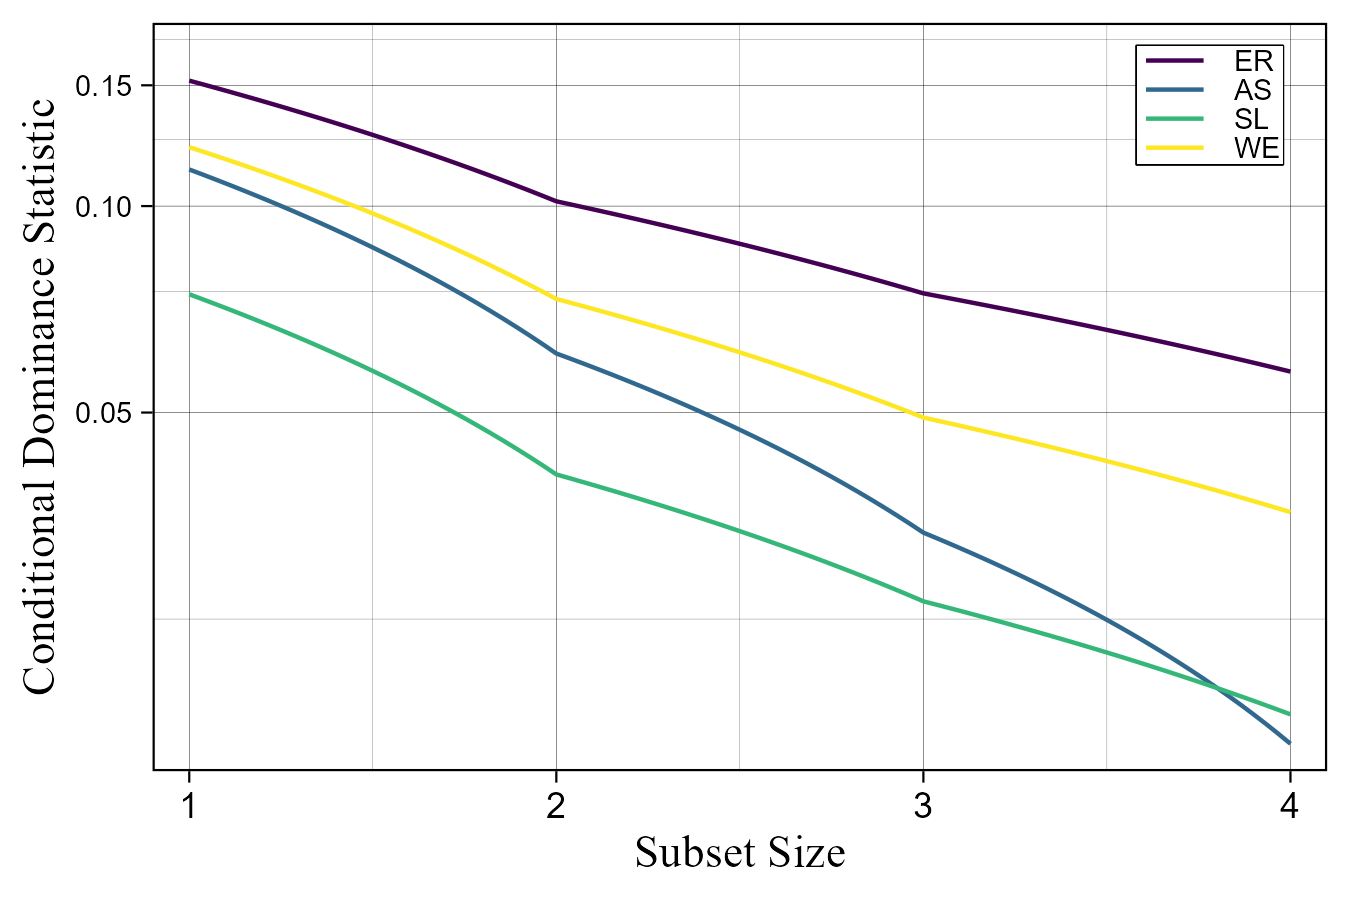
\includegraphics{condit_gph}
		\label{fg:cdl}
	\end{figure}

	I used a graphical format to depict the conditional dominance statistics' values as this format more clearly conveys the dominance designations between IVs than does a table of values. 
	In the graphic, the orientation of each IV's conditional dominance statistic trendline relative to other IVs trendlines represented the information conveyed by Equation \ref{eq:cdldom}.
	Specifically, when an IVs conditional dominance trendline was always above another IV's conditional dominance trendline, the IV that was above conditionally dominated the one below.
	
	The trendlines in Figure \ref{fg:cdl} confirmed the complete dominance results in that equipment reliability's trendline was above the trendlines for the other three IVs indicating that it conditionally dominated each of them.
	Similarly, work experience's trendline was above skill level's trendline consistent with the complete dominance results.
	In addition, work experience's trendline was above assistant staffing's trendline indicating that it conditionally dominated assistant staffing.
	Although work experience did not explain more information than assistant staffing in all comparable models (see $SJ \sim AS + SL$ versus $SJ \sim SL + WE$'s in Table \ref{tab:r2sub}), when considering the average information explained given inclusion order, work experience produced bigger increments to the $R^2_{DEV}$ than did assistant staffing levels. 
	As such, work experience's dominance of assistant staffing was model dependent, but not generally dependent on IV inclusion order.
	
	The last two IVs did not result in conditional dominance designation as assistant staffing failed to conditionally dominate skill level given skill level's conditional dominance statistic when included last in the model (i.e., at subset size 4) was larger than assistant staffing's statistic when included last in the model.
	These conditional dominance results further reinforce the idea that attempting to rank these IVs is not straightforward and their contributions to prediction depend on the order of their inclusion in the model. 
	
	Given that no complete or conditional dominance designations were possible for comparing assistant staffing with skill level, I proceeded to evaluate the general dominance designations between these variables. 
	The general dominance statistics for each tailoring shop IV was computed using Equation \ref{eq:genst} as reported in Table \ref{tab:gen}.
	
	\begin{table}[h!]
		\centering
		\caption{\centering General Dominance Statistics}
		\begin{tabular}{l|r}
			\hline 
			$ER$ & $0.0965$ \\ 
			$AS$ & $0.0560$ \\ 
			$SL$ & $0.0399$ \\ 
			$WE$ & $0.0700$ \\ 
			\hline 
		\end{tabular}
		\label{tab:gen}
	\end{table}

	Evaluating the general dominance designations determined by the general dominance statistics in Table \ref{tab:gen} using Equation \ref{eq:gendom} again showed that equipment reliability dominated each other variable and that work experience dominated skill level and assistant staffing. 
	A useful addition that general dominance designations added was in determining general dominance between assitant staffing and skill level.
	The general dominance designations then added to the previous dominance results in that they were the final component needed to construct an importance hierarchy among the IVs.
	In combination, the results across all three dominance designations resulted in a clear rank ordering of the tailoring shop IVs in predicting sport jackets: equipment reliability was most important followed by work experience, then assistant staffing, and skill level was least important.
	
	In conclusion, the DA results have built on and extended the coefficient reporting in Table \ref{tab:poisreg} by adding additional information about each of the tailoring shop IVs' predictions.
	In particular, the dominance results offered conclusive evidence for differences between IVs in their ability to explain variation or information in the sport jacket production variable. 
	The DA results supported the inference about the predictive usefulness of equipment reliability given its large IRR value. 
	The DA results showed that, regardless of the order in which equipment reliability might be included in the model, it always produced the biggest increment to the $R^2_{DEV}$. 
	In addition, equipment reliability was associated with nearly one-third (i.e., $\frac{.0965}{.2624} \approx \frac{1}{3}$) of the explained information in sport jackets.
	The DA results also provided useful contextualization of work experience, assistant staffing levels, and skill level.
	These three IVs obtained similar IRR values, each within .01 of one another, which made their dominance hierarchy less easy to guess at the outset.
	The dominance designations obtained showed that the hierarchy between these variables was indeed more nuanced as work experience completely dominated only skill level and conditionally dominated assistant staffing levels. 
	Moreover, assistant staffing levels only generally dominated skill level.
	The DA results then provided useful additional information to a researcher about the differences in strength of prediction between these IVs that would not be possible to have obtained only with their IRR values.
	
\section{Discussion}

	In this manuscript I have recommended a methodology for determining the relative importance of IVs in CRMs.
	I recommend the DA methodology as an approach that is comprehensive in the information it provides about IV's prediction and, when using an appropriate fit statistic such as the $R^2_{DEV}$, can provide information analogous to the explained variance $R^2$ using the LRM.
	
	I have also walked the reader through an example data analysis applying PR to simulated data. 
	In walking the reader through this example, I use the recommended DA with $R^2_{DEV}$ fit statistic approach to evaluate the relative importance of four IVs.
	This walk through of the DA has focused on the utilization of different levels of DA designation stringency and how these different levels offer different weights of evidence for the importance of the IVs over one another in predicting the count DV.
	
	By combining these two topics, this manuscript picks up where Blevins et al. \parencite*{blevins2015count} had left off by recommending the use of DA as a postestimation method to better understand CRM predictions.
	Specifically, I recommend consulting Blevins et al's work when choosing to implement a CRM as their decision flowchart can help you to choose the most appropriate CRM given the nature of your data and follow the estimation of the CRM with a DA to more better contextualize the predictions made by each IV.
	
	In this manuscript I have discussed many key considerations for researchers contemplating implementing DA in using CRMs, but I acknowledge that several relevant topics have not been included.
	Before closing, I discuss some noteworthy limitations and additional extensions of this work.
	
	\subsection{Limitations and Future Directions}
	
	In this work, I use only simulated data in the empirical examples.
	The use of simulated data was an intentional choice to avoid the need to work through many of the decision points outlined by Blevins et al. \parencite*{blevins2015count} related to the selection of an appropriate CRM as I know the DVs are distibuted as Poisson or negative Binomial.
	I acknowledge that the use of the simulated data adds additional complexity to following along with the methodology in the online supplement.
	That said, all the procedures used to simulate the various count DVs are fully replicable, well-documented, and available as a markdown that can be used by interested readers with a working knowledge of R \parencite{R}.
	In addition, I acknowledge that only reporting the results from the PR models is a limitation.
	The PR and NBR results were very similar and, in my view, including the NBR results would not meaningfully add to the manucscript's narrative.
	Although the NBR model's results are not in the manuscript, I have included the NBR results in the supplement for interested readers.
	
	Prior work on DA has recommended that researchers use bootstrapping to estimate the reproduce-ability of dominance designations \parencite{azen2003dominance}. 
	Bootstrapping the CRM-based dominance statistics and designations is also possible but was not examined in the present work.
	Although I have not provided an example of bootstrap reproduce-ability in this work, evaluating the bootstrap reproduce-ability of dominance designations is a useful and important practice.
	Evaluating reproduce-ability allows researchers assess a level of confidence that specific designations between IVs will hold under resampling.
	Thus, like standard hypothesis testing, evaluating bootstrap reproduce-ability can allow a researcher to better determine whether a set of dominance designations between IVs in a CRM are likely to generalize beyond the sample at hand.
	
	In addition, zero inflation is commonly observed of count DVs.  
	Zero inflation is a condition where the distribution of the count DV has more 0s than would be expected given a standard Poisson or negative Binomail distribution and requires the use of specialized models \parencite[e.g.,][]{blevins2015count, bhaskar2023regression}. 
	Cameron and Windmeijer \parencite*{cameron1996r} discuss the application of the $R^2_{DEV}$ to zero-inflated CRMs and, thus, a DA methodology based on the same general approach as discussed above could be applied to zero-inflated CRMs.
	One additional complication that arises with considering how to determine importance with zero-inflated CRMs is that these models encompass two predictive processes. 
	The first process is the standard count generating process whereby IVs increase or decrease DV counts.
	The second is an "opt out" process whereby IVs increase or decrease the likelihood of the count being 0.
	These two processes add complexity in that they can be modeled differently. 
	Any one IV can predict the count generating process, the opting out process, or both.
	When using a DA with zero-inflated CRMs, I recommend the researcher consider whether they are truly interested in determining the importance of IVs or are actually interested in determining the importance of parameter estimates \parencite{luchman2020relative}. 
	The key difference between the two perspectives is that, if one IV is included in both the count and opt out process, the IV approach would ascribe the IV a single set of dominance statistic designations whereas the parameter estimate perspective would break the designations into one focused on the IV's effect in the count process and, separately, the IV's effect in the opt out process.
	
	\subsection{Conclusion}
	
	DA is a useful post-estimation methodology for determining the importance of IVs in statistical models such as CRMs.
	This manuscript has provided a recommended methodology for extending DA to CRMs and offered an extensive data analytic example focusing on the interpretation of DA statistics and designations with simulated data.
	In combination, the conceptual discussion of DA and CRMs when paired with the empirical example in this paper, will provide scientists with useful tools they can use to better understand the results of CRMs they estimate in support of research questions with count data.

\printbibliography
	
\end{document}

input{CountDominance.bbl}